
\section{Annotation}
\label{sec:annotation}

Semantic Annotations describe the observation model contained in a
data object. The Annotation serves as a template for constructing a
fully fleshed OBOE model of the [usually tabular] data. Less formal
descriptions of the data attributes are often included in traditional
metadata formats like EML. while there is some overlap between these
two mechanisms - particularly with respect to measurement standards or
units - semantic concepts applied to each attribute have the benefit
of placing the descriptive burden on the ontology from which the
concepts are drawn. Because the Annotation represents a potentially
subjective perspective on the data, they are stored independently as
XML; the former referencing the latter.

The Annotation structure largely mirrors the core classes in
OBOE. Observations are composed of Measurements of a specific Entity
and are represented by a collection of Characteristics (usually just
one) collected using a defined Protocol and Standard (i.e. unit).
Tablular data object attributes are mapped to a Measurement such that
a collection of attributes usually pertain to the Entity of a shared
Observation (\figref{fig:kelp-mass-model}). These Observtions can
provide context for other Observations such that the structure of the
observational data model and collection paradigm are formally
represented in the Annotation.

\begin{figure}
  \centering
  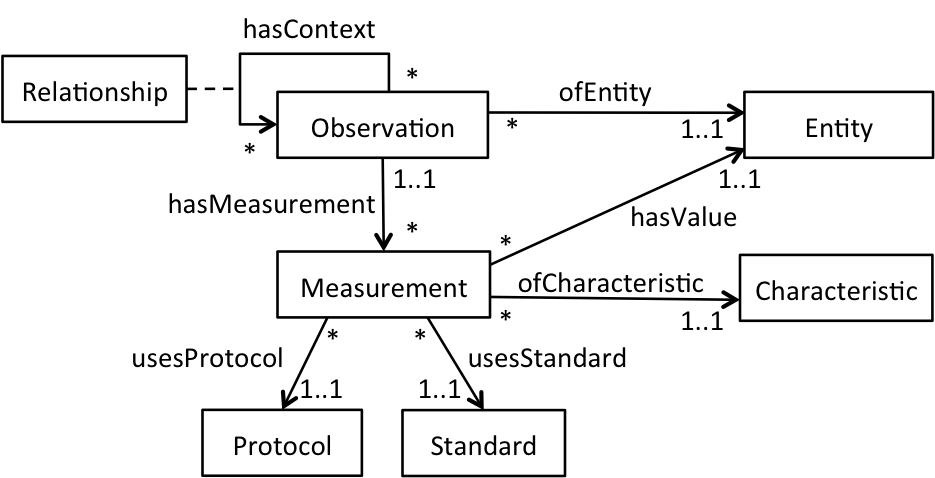
\includegraphics[width=0.5\textwidth]{images/oboe}
  \caption{The main classes and properties of the extensible
    observation ontology (OBOE). While shown using UML, the model is
    defined using OWL-DL.}
  \label{fig:oboe}
\end{figure}

\begin{figure}
\centering
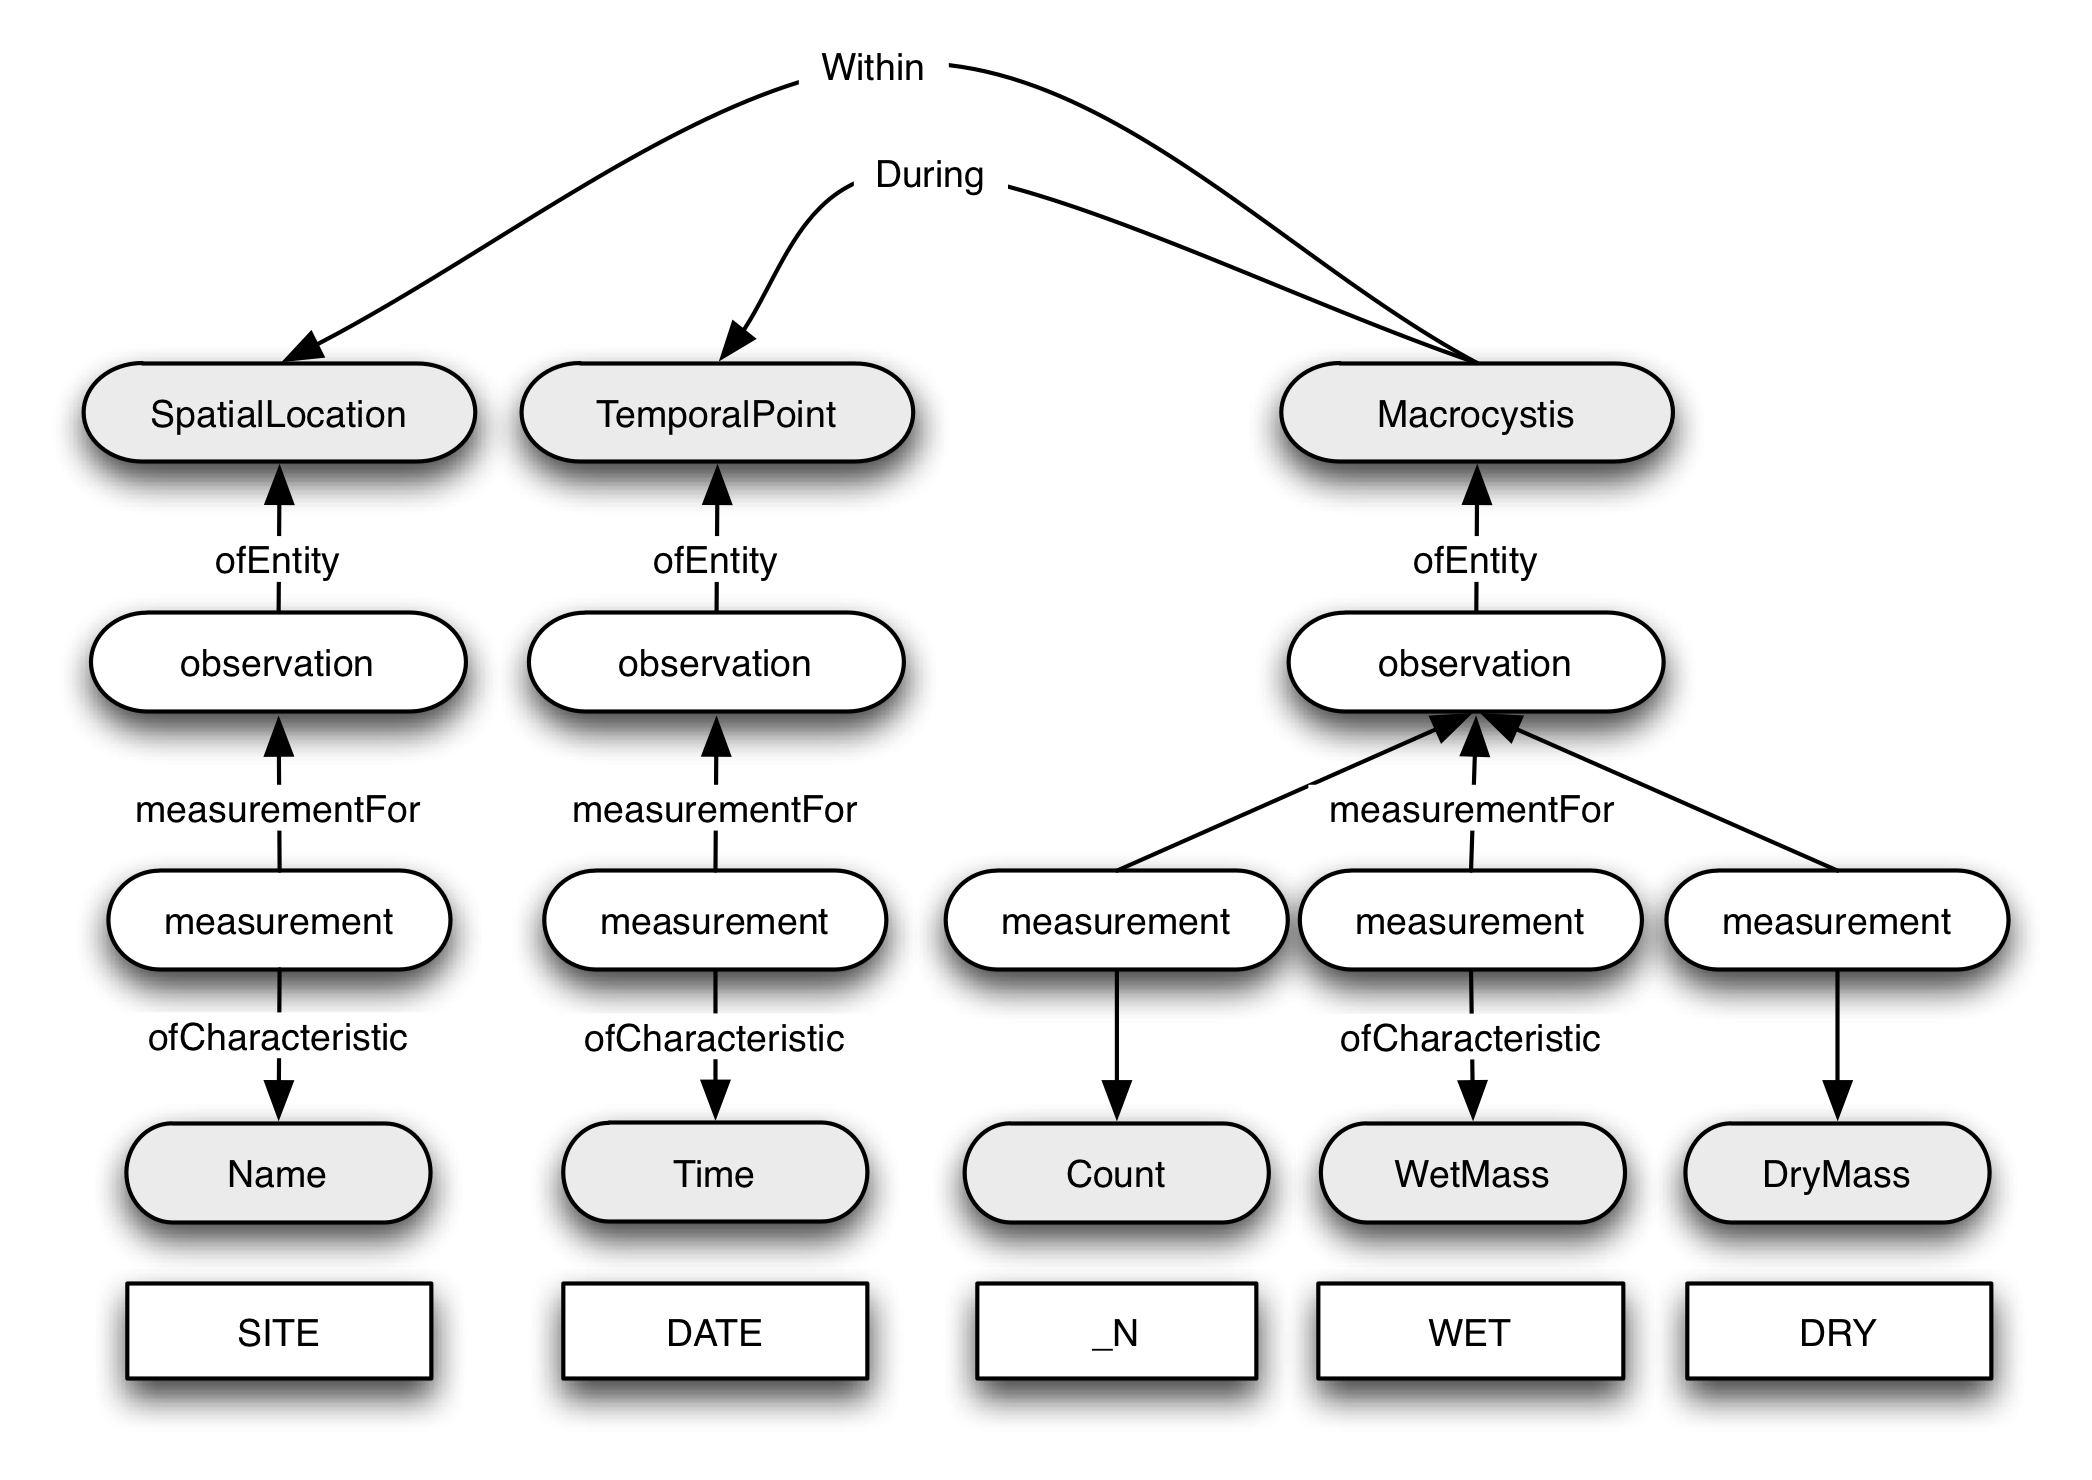
\includegraphics[width=0.5\textwidth]{images/kelp-mass-model.png}
\caption{Partial OBOE Annotation for Kelp sampling data. Shaded nodes represent ontological concepts; rectangular nodes are data table attibutes mapped to OBOE characteristics.}
\label{fig:kelp-mass-model}
\end{figure}

%%% Local Variables: 
%%% mode: latex
%%% TeX-master: "main"
%%% End: 
